% =====================================================================
%  Escala -- Fire Station Shift Management Platform
%  Sprint 1 - Idea Presentation and Progress Status Report
%  LABDSOF 2026/27 -- ISEP
%
%  Compile with pdfLaTeX, twice (contents, lists and links):
%      pdflatex report.tex
%  Images are expected in ./images
% =====================================================================
\documentclass[11pt,a4paper]{article}

% ---------------------------------------------------------------- fonts
\usepackage[T1]{fontenc}
\usepackage[utf8]{inputenc}
\usepackage{textcomp}
\usepackage{libertine}            % same typeface as the cover

% --------------------------------------------------------------- layout
\usepackage[a4paper,margin=2.5cm]{geometry}
\usepackage{pdflscape}
\usepackage{xcolor}
\usepackage{graphicx}
\usepackage{array,tabularx,xltabular,colortbl}
\usepackage{enumitem}
\usepackage{fancyhdr}
\usepackage{microtype}
\usepackage{tikz}
\usepackage{caption}
\usepackage[titles]{tocloft}
\usepackage[hidelinks]{hyperref}
\hypersetup{
  pdftitle={Escala -- Sprint 1 - Idea Presentation and Progress Status Report},
  pdfauthor={Diogo Pereira, Diogo Sousa, Pedro Costa, Diogo Costa}
}

\setlength{\parskip}{0.6em}
\setlength{\parindent}{0pt}

% every chapter (and each of the contents/lists) starts on a new page
\let\oldsection\section
\renewcommand{\section}{\clearpage\oldsection}

% --------------------------------------------- contents and the lists
% compact entries: no paragraph skip between lines, small gaps
\setlength{\cftparskip}{0pt}
\setlength{\cftbeforesecskip}{6pt}
\setlength{\cftbeforesubsecskip}{0pt}
\setlength{\cftbeforefigskip}{2pt}
\setlength{\cftbeforetabskip}{2pt}

% -------------------------------------------------------- page numbers
% Page number centred at the bottom, no header.
\pagestyle{plain}

% Landscape pages: pdflscape rotates only the text body, so the page number
% is drawn rotated at the middle of the long edge that ends up at the bottom.
\fancypagestyle{landscapeplain}{%
  \fancyhf{}\renewcommand{\headrulewidth}{0pt}%
  \fancyhead[C]{%
    \begin{tikzpicture}[remember picture, overlay]
      \node[rotate=90, anchor=base] at ([xshift=-28pt]current page.east) {\thepage};
    \end{tikzpicture}}}

% landscape pages use smaller margins so the diagrams and templates are larger
\newenvironment{widepage}
  {\newgeometry{margin=1.5cm}\begin{landscape}\thispagestyle{landscapeplain}}
  {\end{landscape}\restoregeometry}

% ------------------------------------------------------------ captions
\captionsetup{font=normalsize, labelfont=bf, justification=centering, skip=6pt}
\captionsetup[table]{position=below}
% captions of multi-page tables span the full text width
\setlength{\LTcapwidth}{\textwidth}
\newcommand{\tabcap}[1]{\captionof{table}{#1}}

% ---------------------------------------------------------------- lists
\setlist[itemize]{itemsep=2pt, topsep=4pt, parsep=0pt}

% --------------------------------------------------------------- tables
% Table design (from table-example.png): dark navy header row with small
% white uppercase labels, a light grey-blue first column with bold labels,
% white body cells with orange-red bullets, and a light grey frame and row
% lines. No line between the first and second columns; tables with three
% or more columns keep thin lines between the other columns.
\definecolor{headnavy}{HTML}{1E2533}
\definecolor{firstcol}{HTML}{F4F6F9}
\definecolor{tableline}{HTML}{D5DAE1}
\definecolor{phasegrey}{HTML}{E4E8EE}
\definecolor{bulletred}{HTML}{C4532D}
\newcolumntype{L}{>{\raggedright\arraybackslash}X}
\newcolumntype{P}[1]{>{\raggedright\arraybackslash}p{#1}}
% first column: shaded, bold
\newcolumntype{B}[1]{>{\columncolor{firstcol}\raggedright\arraybackslash\bfseries}p{#1}}
% first column: shaded, regular weight, flexible width
\newcolumntype{F}{>{\columncolor{firstcol}\raggedright\arraybackslash}X}
\renewcommand{\arraystretch}{1.6}
\setlength{\tabcolsep}{8pt}
\setlength{\arrayrulewidth}{0.8pt}
\AtBeginDocument{\arrayrulecolor{tableline}}
% header row: \headrow first, then \hd{...} cells
\newcommand{\headrow}{\rowcolor{headnavy}}
\newcommand{\hd}[1]{\leavevmode{\color{white}\footnotesize\bfseries\textls[80]{\MakeUppercase{#1}}}}
% line under the header row
\newcommand{\hdrule}{\hline}

% bullet list inside a table cell (top-aligned with the rest of the row)
\newcommand{\cellitems}[1]{%
  \begin{minipage}[t]{\linewidth}\raggedright
    \begin{itemize}[nosep, leftmargin=1.1em, label={\color{bulletred}\textbullet}]
      #1
    \end{itemize}\vspace{4pt}
  \end{minipage}}

% persona cell: avatar, name, short profile and the group represented
\newcommand{\personacell}[4]{%
  \begin{minipage}[t]{\linewidth}\centering
    % glue first: the top of the cell is the row's reference point; pull the
    % avatar up so its top lines up with the first line of the other columns
    \vspace{-6pt}
    \includegraphics[width=1.4cm]{images/avatar-#1.pdf}\par\vspace{2pt}
    \textbf{#2}\par
    {\footnotesize #3}\par\vspace{2pt}
    {\footnotesize\textit{#4}}\par\vspace{4pt}
  \end{minipage}}

\begin{document}

% =====================================================================
%  COVER
% =====================================================================
\begin{titlepage}
  \centering\color{black}
  \vspace*{58pt}
  
\includegraphics[width=199pt]{images/isep-logo.png}\par
  \vspace{62pt}
  {\fontsize{34}{40}\selectfont\bfseries Escala\par}
  \vspace{6pt}
  {\fontsize{17.28}{21.6}\selectfont Fire Station Shift Management Platform\par}
  \vspace{38pt}
  {\fontsize{14.4}{20}\selectfont\bfseries
    \underline{Sprint 1 -- Idea Presentation}\\
    \underline{and Progress Status Report}\par}
  \vspace{13pt}
  {\fontsize{14.4}{18}\selectfont LABDSOF 2026/27\par}
  \vspace{70pt}
  {\fontsize{17.28}{21.6}\selectfont\bfseries Masters in Software Engineering\par}
  \vspace{8pt}
  {\fontsize{14.4}{18}\selectfont School of Engineering -- Polytechnic Institute of Porto\par}
  \vfill
  % team table (booktabs-style rules, black)
  {\fontsize{12}{14.5}\selectfont
   \renewcommand{\arraystretch}{1.12}%
   \begin{tabular}{@{\hspace{6pt}}l@{\hspace{40pt}}c@{\hspace{6pt}}}
     \noalign{\hrule height 0.8pt}\noalign{\vspace{3pt}}
     \textbf{Name} & \textbf{Student no.} \\
     \noalign{\vspace{2pt}\hrule height 0.5pt\vspace{3pt}}
     Diogo Pereira & 1221137 \\
     Diogo Sousa   & 1250505 \\
     Pedro Costa   & 1211439 \\
     Diogo Costa   & 1211514 \\
     \noalign{\vspace{3pt}\hrule height 0.8pt}
   \end{tabular}\par}
  \vspace{48pt}
  {\fontsize{14.4}{18}\selectfont Porto, 10 October 2026\par}
\end{titlepage}
\setcounter{page}{2}

% =====================================================================
%  CONTENTS, LIST OF FIGURES, LIST OF TABLES  (one page each)
% =====================================================================
\tableofcontents
\listoffigures
\listoftables

% =====================================================================
%  1  PROBLEM AND OPPORTUNITY
% =====================================================================
\section{Problem and Opportunity}

\subsection{Problem Context}
The station's weekly schedule lives on paper. The supervisor defines the shifts and tracks,
by hand, the minimum and maximum weekly hours of each member. The schedule is then edited in
Excel and printed, and some members post a photo of it in the station's WhatsApp group.

Every change to the schedule means editing and reprinting it. This process causes three
main problems:
\begin{itemize}
  \item \textbf{Checking the schedule:} professional firefighters, volunteers and cadets have
        to go to the station to check their current schedule, or depend on other members
        posting updates in the WhatsApp group. Not every update is posted, so members often
        rely on an outdated schedule.
  \item \textbf{Keeping track of changes:} it is hard for the supervisor to follow every
        change, especially the shift extensions caused by emergencies and the swaps that
        members request. Some extensions and swaps are lost along the way, or never reach him
        at all.
  \item \textbf{Requesting swaps:} volunteers and cadets have to fit their shifts around their
        jobs, school and personal lives. To swap a shift, they must find another member to
        swap with and report the swap to the supervisor. Often only one of them reports it,
        and the other has no easy way of knowing whether the change was approved.
\end{itemize}

Together, these problems have led to a high turnover of volunteers and cadets.

\subsection{Opportunity}
There is an opportunity to implement \textbf{Escala}, a shift management app built for the
station, whose need was raised by the cadets, volunteers and former members themselves.
Escala addresses each of the problems above:
\begin{itemize}
  \item \textbf{Checking the schedule:} a single, always up-to-date schedule, available on
        members' phones and on the station computers, replaces the printed sheet and the
        WhatsApp photos. Everyone is notified of the changes that affect them, so nobody has
        to go to the station or wait for an update that may never be posted.
  \item \textbf{Keeping track of changes:} every change is made and recorded in the app. The
        supervisor builds the weekly schedule with each member's availability, hours and
        limits in view, and publishes changes without reprinting. Professional firefighters
        register their extensions and call-outs themselves after the emergency, for the
        supervisor to review and approve, so no hours are lost.
  \item \textbf{Requesting swaps:} members mark their availability in advance and request
        swaps among themselves in the app. Both members see the result straight away, and
        the swap is logged for the supervisor.
\end{itemize}

Escala also gives dispatchers an on-shift board showing who is on shift at any moment,
alongside the station's existing dispatch app. Since senior staff have little experience
with technology, it is designed to be used from day one, without training. By making the
schedule easier to follow and to fit around members' lives, Escala aims to reduce the
turnover of volunteers and cadets.

\subsection{Target Community}\label{sec:community}
The target community is a Portuguese fire brigade association (\emph{Associação
Humanitária de Bombeiros}). One of its stations will be the pilot, with development funded
by the municipality. Later, Escala can reach other fire brigades and humanitarian
organisations that rely on volunteer shifts.

Within the station, the groups affected by the current schedule, and their problems, are
listed in Table~\ref{tab:affected}.

{\small
\begin{xltabular}{\linewidth}{|B{3.6cm}L|}
  \hline
  \headrow\hd{Group} & \hd{Problems} \\ \hdrule
  \endhead
  Professional firefighters &
    \cellitems{
      \item Emergencies extend shifts or cause night call-outs
      \item Extensions can't be reported during the emergency, and the supervisor has often left by the time they return
      \item Extra hours are miscounted or lost
      \item The weekly day off is only known when the schedule is posted
    } \\ \hline
  Volunteers and cadets &
    \cellitems{
      \item Limited, irregular availability
      \item To know the final schedule they must go to the station or wait for a WhatsApp photo
      \item Not every update is posted on WhatsApp
      \item The schedule clashes with school, jobs and personal life
    } \\ \hline
  Supervisor &
    \cellitems{
      \item Builds the schedule in Excel
      \item Tracks each member's minimum hours and weekly limit by hand
      \item Every change means editing and reprinting the schedule
      \item Swaps and extensions made after hours, and the paper sheet for extensions, are hard to track and often go missing
    } \\ \hline
  Station chief &
    \cellitems{
      \item Hard to know who is on shift at a given moment
      \item Hard to find times when enough cadets and volunteers can attend training
    } \\ \hline
  Dispatchers &
    \cellitems{
      \item The dispatch app shows who \emph{has been dispatched}, not who is \emph{on shift}
      \item They have to rely on the Excel list to guess who is on shift
    } \\ \hline
  \caption{Groups affected by the current schedule and their problems}\label{tab:affected}
\end{xltabular}}

\textbf{Note:} Senior staff, such as the supervisor and the station chief, have little
familiarity with technology. Any tool must therefore be simple enough for them to adopt
quickly and become part of the station's daily operations from day one, without training.

% ---------------------------------------------------------------------
\begin{widepage}
  \subsection{Product Vision Board}
  \centering
  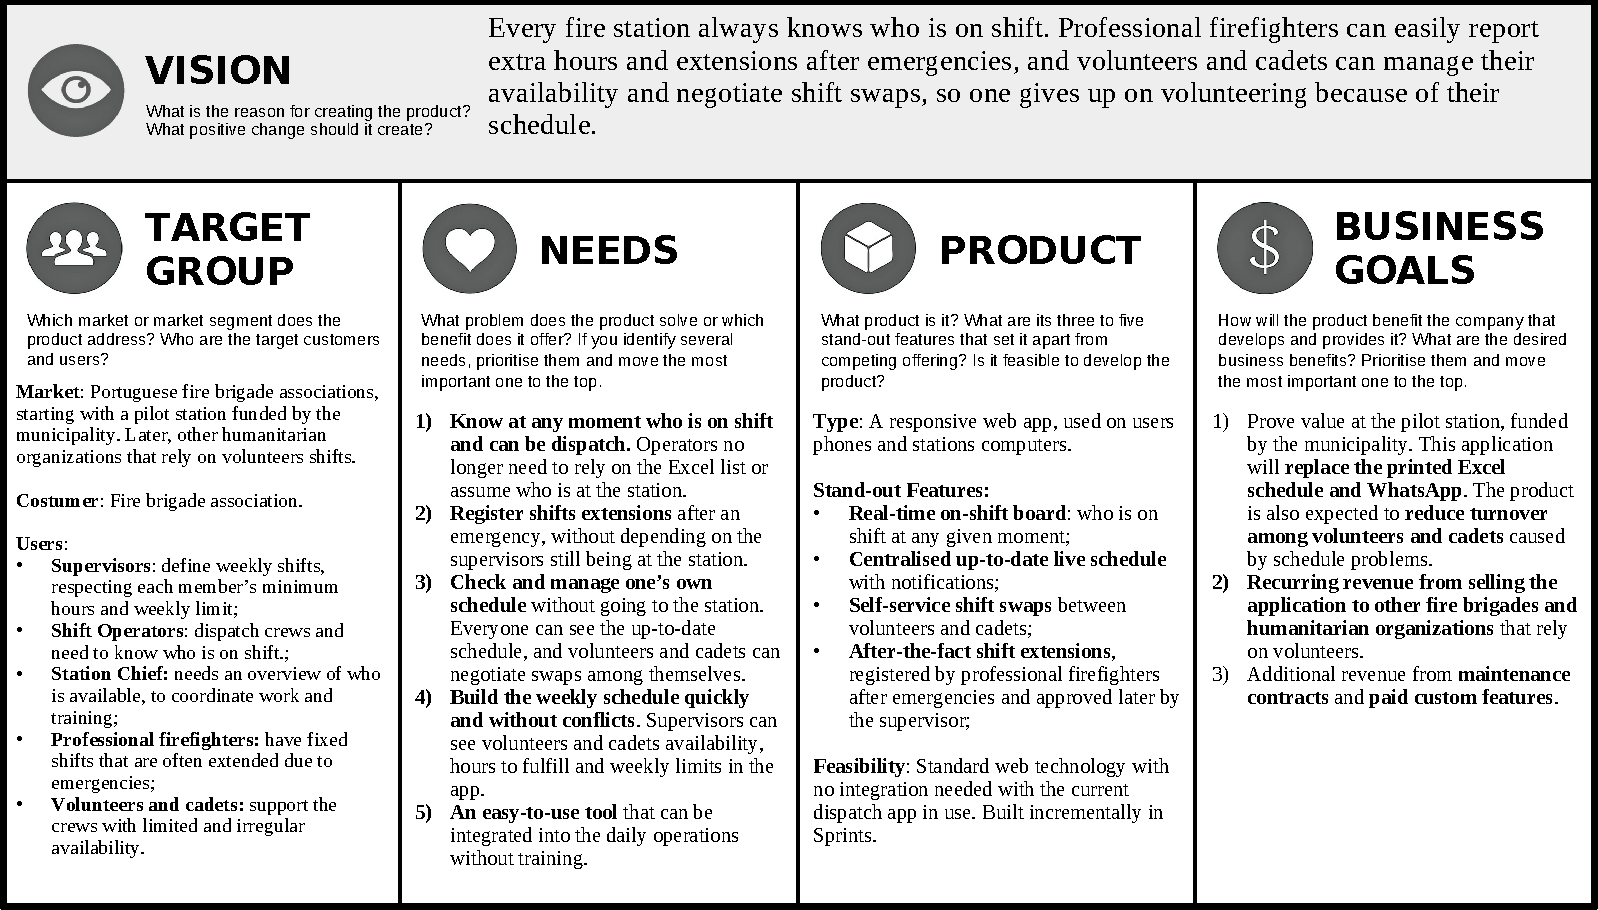
\includegraphics[width=\linewidth,height=0.86\textheight,keepaspectratio]{images/vision-board.pdf}
  \captionof{figure}{Product Vision Board}\label{fig:vision-board}
\end{widepage}

% ---------------------------------------------------------------------
\subsection{Stakeholder Map}
\begin{center}
\begin{tabularx}{\linewidth}{|B{3.3cm}L|P{1.75cm}|P{1.95cm}|P{2.6cm}|}
  \hline
  \headrow\hd{Stakeholder} & \hd{Relation} & \hd{Interest} & \hd{Influence} & \hd{Engagement} \\ \hdrule
  Supervisor & Primary user: builds the schedule & High & High & Manage closely \\ \hline
  Shift chief (\emph{chefe de piquete}), from Firefighter 1st class up
    & Approves swaps, sees who is present before the shift and decides reinforcements & High & Medium & Manage closely \\ \hline
  Station chief & Decision maker on adoption (decides whether the corps adopts the app) & Medium & High & Keep satisfied \\ \hline
  Volunteers and cadets & Users & High & Medium & Involve in tests \\ \hline
  Professional firefighters & Users & High & Medium & Involve in tests \\ \hline
  Dispatchers & See who is on duty (read-only) & Medium & Low & Keep informed \\ \hline
  Fire brigade association & Customer & Medium & High & Keep satisfied \\ \hline
  Municipality & Possible funder (assumption) & Low & High & Monitor \\ \hline
  Existing dispatch app & Neighbouring system, no integration & Low & Low & Monitor \\ \hline
  IPMA & External data source (fire risk) & Low & Low & Monitor \\ \hline
\end{tabularx}
\tabcap{Stakeholder map}\label{tab:stakeholders}
\end{center}

% =====================================================================
%  2  PERSONAS
% =====================================================================
\section{Personas}

\subsection{Target Customers and Users}
\textbf{Customer:}
\begin{itemize}
  \item Fire brigade associations (\emph{Associações Humanitárias de Bombeiros})
  \item Starting with the pilot station, whose development is funded by the municipality
\end{itemize}

\textbf{Users:}
\begin{itemize}
  \item Supervisors
  \item Dispatchers
  \item The station chief
  \item Professional firefighters
  \item Volunteers and cadets
\end{itemize}

\clearpage  % keep the personas table on a single page
\subsection{The Personas}
Each persona stands for one of the target user groups. Table~\ref{tab:personas} gives a
brief summary of the user personas: who they are, their main current problems and what
they want solved. The full persona templates follow.

{\small
\begin{xltabular}{\linewidth}{|>{\columncolor{firstcol}\centering\arraybackslash}p{3.3cm}L|L|}
  \hline
  \headrow\hd{Persona} & \hd{Current problems} & \hd{Wants solved} \\ \hdrule
  \endhead
  \personacell{bernardino-santos}{Bernardino Santos}{Supervisor, 59}{Supervisors}
  &
    \cellitems{
      \item Every change means editing and reprinting the Excel schedule
      \item Changes and extensions made after he leaves get lost
      \item Tracks minimum hours and weekly limits by hand
    }
  &
    \cellitems{
      \item See availability, hours left and weekly limits
      \item Update the schedule without reprinting it
      \item Review and approve extensions registered in the app
    } \\ \hline
  \personacell{rui-carvalho}{Rui Carvalho}{Station chief, 52}{Station command}
  &
    \cellitems{
      \item Hard to find times when enough people can attend training
      \item No quick overview of who is on shift
      \item Couldn't learn Google Calendar or Notion
    }
  &
    \cellitems{
      \item Fewer volunteers and cadets quitting
      \item See at a glance who is on shift and available
      \item Plan training around known availability
    } \\ \hline
  \personacell{pedro-pacheco}{Pedro Pacheco}{Professional firefighter, 31}{Professional firefighters}
  &
    \cellitems{
      \item Extra hours are hard to report and often go missing
      \item Only learns his day off on Monday, at the station
      \item Confirming a swap means going to the station or relying on WhatsApp
    }
  &
    \cellitems{
      \item Register every extra hour himself
      \item Know his schedule and day off in advance
      \item Check schedules on his phone when asked to swap
    } \\ \hline
  \personacell{diogo-ribeiro}{Diogo Ribeiro}{Volunteer, 23}{Volunteers and cadets}
  &
    \cellitems{
      \item Depends on WhatsApp to know about changes
      \item Misses updates that are never posted
      \item Station shifts clash with his Red Cross Sundays
    }
  &
    \cellitems{
      \item Know his schedule at any moment, on his phone
      \item Set availability around his job and Red Cross shifts
      \item Swap shifts and see the update straight away
    } \\ \hline
  \personacell{rita-machado}{Rita Machado}{Former volunteer, 25}{Volunteers who quit}
  &
    \cellitems{
      \item Irregular ICU shifts with frequent changes
      \item Relied on colleagues to report her swaps
      \item Was scheduled on top of her ICU shifts
    }
  &
    \cellitems{
      \item Mark when she isn't available, and update it easily
      \item Request swaps from her phone and see them confirmed
    } \\ \hline
  \caption{Brief summary of the user personas}\label{tab:personas}
\end{xltabular}}

% ---------------------------------------------------------------------
% one landscape page holding a single full-page figure
% \bigfigure[label]{heading or empty}{file}{caption}
\newcommand{\bigfigure}[4][]{%
  \begin{widepage}
    #2
    \centering
    \includegraphics[width=\linewidth,height=0.86\textheight,keepaspectratio]{images/#3}
    \captionof{figure}{#4}\if\relax\detokenize{#1}\relax\else\label{#1}\fi
  \end{widepage}}

\bigfigure{\subsection{Persona Templates}}{persona-bernardino-santos.pdf}{Persona template -- Bernardino Santos, supervisor}
\bigfigure{}{persona-rui-carvalho.pdf}{Persona template -- Rui Carvalho, station chief}
\bigfigure{}{persona-pedro-pacheco.pdf}{Persona template -- Pedro Pacheco, professional firefighter}
\bigfigure{}{persona-diogo-ribeiro.pdf}{Persona template -- Diogo Ribeiro, volunteer}
\bigfigure{}{persona-rita-machado.pdf}{Persona template -- Rita Machado, former volunteer}

% =====================================================================
%  3  ALTERNATIVES
% =====================================================================
\section{Alternatives}\label{sec:alternatives}
The station has already tried Google Calendar and Notion to manage the schedule, and
dropped both because they took too long to learn.

\begin{center}
\begin{tabularx}{\linewidth}{|B{3.2cm}L|}
  \hline
  \headrow\hd{Aspect} & \hd{Google Calendar and Notion} \\ \hdrule
  Learning curve & Took too long to learn and required some technical skill. Senior staff have little experience with technology, and there is no time for training. \\ \hline
  Shift swaps & No shift-swap workflow: every swap would still have to be reported to the supervisor. \\ \hline
  Who is on shift & No view of who is on shift at a given moment. \\ \hline
  Hours & No way to track each member's minimum hours and weekly limit while building the schedule. \\ \hline
\end{tabularx}
\tabcap{Why the tools the station tried failed}\label{tab:alternatives}
\end{center}

These tools were not rejected for missing features alone: the station gave up on them
because senior staff could not learn them quickly enough, and there is no time to train
every member. Simplicity is therefore the deciding factor for adoption. Whatever tool the
station uses must work from the first use, for every member, without training.

% =====================================================================
%  4  VALUE PROPOSITION
% =====================================================================
\section{Value Proposition}

\subsection{What Escala Must Fix}
For fire stations that mix professional firefighters, volunteers and cadets and run their
schedule on a printed Excel sheet, Escala is a shared shift schedule that anyone can use
from day one. It always shows who is on shift and lets members manage their availability,
swaps and extensions themselves. Unlike generic scheduling apps or emergency-services tools
designed for other markets, it needs no training and fits how Portuguese stations actually
work.

For the station, the value lies in time and reliability. Table~\ref{tab:value} shows what
Escala changes for each group.

\begin{center}
\begin{tabularx}{\linewidth}{|B{4.6cm}L|}
  \hline
  \headrow\hd{User group} & \hd{Value of Escala} \\ \hdrule
  Supervisor &
    \cellitems{
      \item Stops rebuilding and reprinting the schedule
      \item Sees each member's hours and limits without counting them by hand
    } \\ \hline
  Dispatchers &
    \cellitems{
      \item Know at any moment who they can send
    } \\ \hline
  Professional firefighters &
    \cellitems{
      \item No extra hours are lost after an emergency
    } \\ \hline
  Volunteers and cadets &
    \cellitems{
      \item No more trips to the station to check the schedule
      \item No more missed WhatsApp updates, which today lead some of them to give up volunteering
    } \\ \hline
\end{tabularx}
\tabcap{Value of Escala for each user group}\label{tab:value}
\end{center}

The pilot station uses Escala at no cost, as its development is funded by the municipality.
Other institutions pay a subscription per active user, kept low enough for non-profit
associations (indicatively \texteuro 1--3 per user per month).

\clearpage  % keep the heading together with its table
\subsection{Main Features}

\begin{center}
\begin{tabularx}{\linewidth}{|B{4.6cm}L|}
  \hline
  \headrow\hd{User group} & \hd{Main features} \\ \hdrule
  Professional firefighters &
    \cellitems{
      \item Report shift extensions and off-hours shifts (call-outs) after the emergency, for the supervisor to approve
    } \\ \hline
  Professional firefighters, volunteers and cadets &
    \cellitems{
      \item Define their unavailability in advance
      \item Check their schedule on the phone and be notified of every change that affects them
      \item Request and negotiate shift swaps among themselves
    } \\ \hline
  Supervisor &
    \cellitems{
      \item Build the weekly schedule with each member's availability, minimum hours and weekly limit in view
      \item Automatic checks for unavailability, unfilled roles, overlapping shifts and hours above the weekly limit
      \item Publish the schedule, and any later change, without reprinting it
      \item Review, approve or reject extensions and off-hours shifts
      \item See every change, swap and extension in the change log
    } \\ \hline
  Station chief &
    \cellitems{
      \item See who is on shift and who is available, to plan training sessions
    } \\ \hline
  Dispatchers &
    \cellitems{
      \item On-shift board showing who is on shift at any moment, ready for dispatch
      \item Complements the existing dispatch app, without integrating with it
    } \\ \hline
\end{tabularx}
\tabcap{Main features of Escala for each user group}\label{tab:features}
\end{center}

\subsection{What Is Essential}
Beyond its features, the following points are essential for Escala to be adopted by the
station, as summarised in Table~\ref{tab:essentials}.

\begin{center}
\begin{tabularx}{\linewidth}{|B{4.6cm}L|}
  \hline
  \headrow\hd{Essential} & \hd{Description} \\ \hdrule
  Usable from the first use &
    \cellitems{
      \item Senior members of the station must be able to adapt quickly
      \item Simple screens, large buttons, few steps, in Portuguese
      \item No training needed
    } \\ \hline
  One central schedule &
    \cellitems{
      \item Always up to date, with real-time updates
      \item The people affected are notified of every change
    } \\ \hline
  Weekly hours tracking &
    \cellitems{
      \item Minimum hours and weekly limit of each member, counted automatically
    } \\ \hline
\end{tabularx}
\tabcap{What is essential for Escala to be adopted}\label{tab:essentials}
\end{center}

% =====================================================================
%  5  USER JOURNEYS
% =====================================================================
\section{User Journeys}
Taking all of the above into account, five principal user journeys were defined, as
summarised in Table~\ref{tab:journeys}.

% journey cell: ID and name (like the persona cell, without the avatar)
\newcommand{\journeycell}[2]{%
  \begin{minipage}[t]{\linewidth}\centering
    \vspace{-2pt}
    {\large\bfseries #1}\par\vspace{2pt}
    {\small #2}\par\vspace{4pt}
  \end{minipage}}

{\small
\begin{xltabular}{\linewidth}{|>{\columncolor{firstcol}\centering\arraybackslash}p{3.3cm}P{3.6cm}|L|}
  \hline
  \headrow\hd{Journey} & \hd{Actors} & \hd{Description} \\ \hdrule
  \endhead
  \journeycell{UJ1}{Plan the weekly schedule}
  &
    \cellitems{\item Professional firefighters, volunteers and cadets \item Supervisor}
  &
    \cellitems{
      \item Members define their unavailability for the next week
      \item The supervisor defines the shifts and the roles each one needs, and fills the schedule manually or automatically
      \item Escala checks for conflicts before the schedule is approved and published
      \item Every member is notified
    } \\ \hline
  \journeycell{UJ2}{Register a shift extension or off-hours shift}
  &
    \cellitems{\item Professional firefighter \item Supervisor}
  &
    \cellitems{
      \item After an emergency, the firefighter registers the extra hours
      \item The supervisor approves them, or rejects them with a reason
      \item The firefighter can ask for one more review
      \item Approved hours update the schedule
    } \\ \hline
  \journeycell{UJ3}{Ask for a shift swap}
  &
    \cellitems{\item Requesting member \item Colleague \item Supervisor (informed only)}
  &
    \cellitems{
      \item A member asks a specific colleague to swap, or publishes the request for anyone
      \item Escala checks that each member can fill the other's role and stays within the weekly limit
      \item Valid swaps update both schedules and appear in the supervisor's change log
    } \\ \hline
  \journeycell{UJ4}{See who is on shift to dispatch}
  &
    \cellitems{\item Dispatcher}
  &
    \cellitems{
      \item The dispatcher opens the on-shift board
      \item Sees who is on shift, with their role and shift end time
      \item Dispatches the crew in the existing dispatch app
    } \\ \hline
  \journeycell{UJ5}{Plan a training session}
  &
    \cellitems{\item Station chief \item Selected members}
  &
    \cellitems{
      \item The station chief picks a shift and the members to train
      \item Escala checks that key roles stay covered on shift
      \item The selected members are notified
    } \\ \hline
  \caption{Principal user journeys}\label{tab:journeys}
\end{xltabular}}

% one journey diagram per landscape page, as large as the page allows
\bigfigure[fig:uj1]{\subsection{User Journey Diagrams}}{journey-UJ1-weekly-schedule.png}{UJ1 -- Plan the weekly schedule}
\bigfigure[fig:uj2]{}{journey-UJ2-shift-extension.png}{UJ2 -- Register a shift extension or off-hours shift}
\bigfigure[fig:uj3]{}{journey-UJ3-shift-swap.png}{UJ3 -- Ask for a shift swap}
\bigfigure[fig:uj4]{}{journey-UJ4-on-shift-board.png}{UJ4 -- See who is on shift to dispatch}
\bigfigure[fig:uj5]{}{journey-UJ5-plan-training.png}{UJ5 -- Plan a training session}

% =====================================================================
%  6  USER WORKFLOWS
% =====================================================================
% heading and intro share the first diagram's landscape page, so the image is a bit shorter
\begin{widepage}
  \section{User Workflows}
  Building on the user journeys, two workflows describe how Escala supports them:
  filling an open slot in the roster (Figure~\ref{fig:wf1}) and blocking an assignment
  when the firefighter has declared unavailability (Figure~\ref{fig:wf2}).\par\medskip
  \centering
  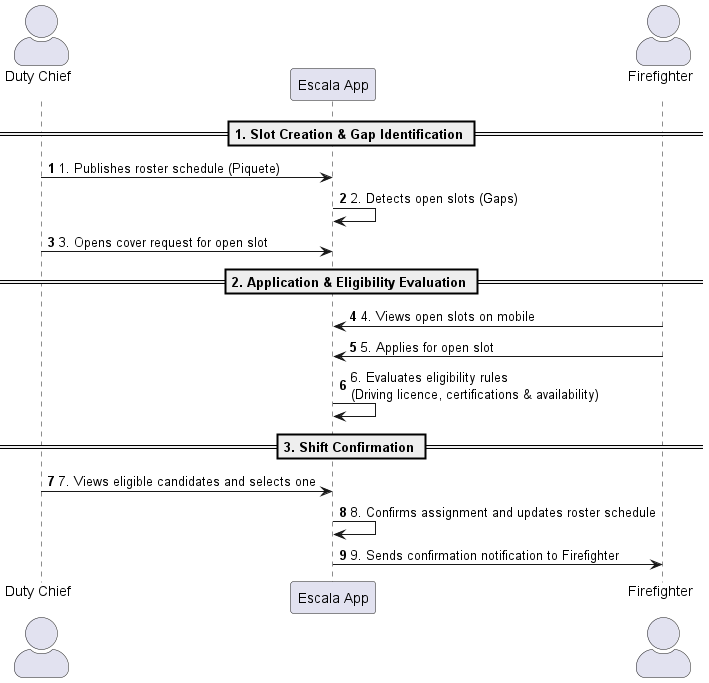
\includegraphics[width=\linewidth,height=0.74\textheight,keepaspectratio]{images/workflow.png}
  \captionof{figure}{Workflow -- Filling an open slot in the roster}\label{fig:wf1}
\end{widepage}
\bigfigure[fig:wf2]{}{workflow_2.png}{Workflow -- Assignment blocked by declared unavailability}

% =====================================================================
%  7  SPRINT 1 - CURRENT STATUS OF THE DELIVERABLES
% =====================================================================
\section{Sprint 1 -- Current Status of the Deliverables}
Table~\ref{tab:deliverables} lists the deliverables requested for the first sprint
(Sprint A), grouped by phase, and the current status of each.

% phase row spanning the whole table
\newcommand{\phaserow}[1]{\multicolumn{3}{|l|}{\cellcolor{phasegrey}\textbf{#1}} \\ \hline}

{\small
\begin{xltabular}{\linewidth}{|FP{2.3cm}|P{5.6cm}|}
  \hline
  \headrow\hd{Deliverable} & \hd{Status} & \hd{Notes} \\ \hdrule
  \endhead
  \phaserow{Phase 1}
  Source control Git repository setup (e.g.\ GitHub, Bitbucket) & \textbf{Done} & GitHub repository created. \\ \hline
  Issue tracking system setup (e.g.\ Jira, GitHub) & \textbf{Done} & Jira project with epics, stories and decisions. \\ \hline
  Agree on a team methodology & \textbf{Done} & Scrum, with a pre-game phase, sprints and a post-game phase. \\ \hline
  Elaborate the Definition of Ready & \textbf{Done} & Documented in Confluence. \\ \hline
  Elaborate the Definition of Done & \textbf{Done} & Documented in Confluence. \\ \hline
  Role identification and assignment & \textbf{Done} & Product Owner, Scrum Master and Developers. \\ \hline
  \phaserow{Phase 2}
  Research on the project domain & \textbf{Done} & Needs of each user group described. \\ \hline
  Research on related works & \textbf{Done} & Alternatives analysed. \\ \hline
  Elaborate questions to customers & \textbf{In progress} & Questions prepared for the station; more personas still to be created. \\ \hline
  Interviews with the customer (or other elicitation techniques) & \textbf{In progress} & Findings used for the personas; notes still to be documented. \\ \hline
  Initial list of functional requirements (epics/features) and NFRs & \textbf{In progress} & Epics in Jira being aligned with the current scope. \\ \hline
  \phaserow{Phase 3}
  Document the functional scope proposal (product vision, user personas, epics, general workflow, domain model) & \textbf{In progress} & Product vision, personas and user journeys done; domain model drafted, to be reviewed by the team; epics being updated. \\ \hline
  Create the Product Backlog & \textbf{In progress} & User stories in Jira being aligned with the current scope. \\ \hline
  Prioritize the backlog with the customer (MoSCoW) & \textbf{Not started} & --- \\ \hline
  Create the Sprint B backlog (ensuring the Definition of Ready) & \textbf{Not started} & --- \\ \hline
  \caption{Sprint A deliverables and their current status}\label{tab:deliverables}
\end{xltabular}}

% status dot: \statusdot{colour}{label}
\definecolor{statusgreen}{HTML}{2E9E55}
\definecolor{statusyellow}{HTML}{E3A812}
\definecolor{statusred}{HTML}{D2423B}
\newcommand{\statusdot}[2]{%
  \mbox{\tikz[baseline=-0.6ex]\fill[#1] (0,0) circle (3.6pt);\hspace{5pt}\textbf{#2}}}

\clearpage  % keep the introduction together with its table
Table~\ref{tab:artifacts} gives the general status of the remaining artifacts for the first
delivery: \statusdot{statusgreen}{green} complete, \statusdot{statusyellow}{yellow} in
progress and \statusdot{statusred}{red} not started.

\begin{center}
\begin{tabularx}{\linewidth}{|B{4.6cm}P{2.6cm}|L|}
  \hline
  \headrow\hd{Artifact} & \hd{Status} & \hd{Notes} \\ \hdrule
  DoR / DoD & \statusdot{statusgreen}{Green} & Definition of Ready and Definition of Done agreed and documented in Confluence. \\ \hline
  Team roles and work process & \statusdot{statusgreen}{Green} & Product Owner, Scrum Master and Developers assigned; Scrum process with working agreements defined. \\ \hline
  Domain model & \statusdot{statusyellow}{Yellow} & Draft done and available in the \texttt{docs} folder of the GitHub repository; still needs a thorough review by the team. \\ \hline
  High-level system architecture & \statusdot{statusgreen}{Green} & Done; available in the \texttt{docs} folder of the GitHub repository. \\ \hline
\end{tabularx}
\tabcap{General status of the remaining artifacts for the first delivery}\label{tab:artifacts}
\end{center}

\end{document}
